% -*- mode: noweb; noweb-default-code-mode: R-mode; -*-
%\VignetteIndexEntry{An R package for fitting probabilistic index models}
%\VignetteKeyword{probabilistic index model, regression}
%\VignetteDepends{pim}
%\VignettePackage{pim}
%documentclass[12pt, a4paper]{article}
\documentclass[12pt]{article}

\usepackage{amsmath}
\usepackage{amssymb}
\usepackage{hyperref}
\usepackage[authoryear,round]{natbib}
\usepackage[utf8]{inputenc}

 
\textwidth=6.2in
\textheight=8.5in
%\parskip=.3cm
\oddsidemargin=.1in
\evensidemargin=.1in
\headheight=-.3in

\newcommand{\prob}[1]{\text{P}\left\{#1\right\}}
\newcommand{\hatprob}[1]{\hat{\text{P}}\left\{#1\right\}}
\newcommand{\I}[1]{\text{I}\left\{#1\right\}}
\newcommand{\leqs}{\preccurlyeq}



\author{Jan De Neve}
\usepackage{Sweave}
\begin{document}
\Sconcordance{concordance:pim.tex:pim.Rnw:%
1 32 1 1 0 119 1 1 2 1 0 2 1 12 0 2 2 1 0 1 3 2 0 1 1 13 0 1 2 14 1 1 2 %
17 0 1 2 1 1 1 2 5 0 1 2 1 1 1 2 7 0 1 1 8 0 1 1 12 0 1 2 8 1 1 2 1 0 1 %
1 12 0 1 2 1 4 3 0 1 1 15 0 1 2 18 1 1 5 4 0 1 1 17 0 1 2 13 1 1 2 4 0 %
1 2 1 8 7 0 1 1 16 0 1 2 23 1 1 2 1 0 3 1 1 3 2 0 1 1 15 0 1 2 21 1}

\title{pim: An R package for fitting probabilistic index models}

\maketitle
\tableofcontents
\section{Introduction}

This document explains and illustrates how the \texttt{pim}-package can be employed to fit a Probabilistic Index Model (PIM). We refer to \cite{Thas2012} for a detailed overview on PIMs. If $(Y,X)$ and $(Y',X')$ are i.i.d. then a PIM is defined as
\begin{equation}\label{pim}
\prob{Y \leqs Y' | X, X'} = m(X,X';\beta) = g^{-1}(Z^T \beta) \quad \text{for} \quad (X,X') \in \mathcal{X},
\end{equation}
with $\prob{Y \leqs Y'} \equiv  \prob{Y < Y'} + \frac{1}{2} \prob{Y = Y'}$. Here $g(\cdot)$ denotes a link function, $Z$ is a covariate vector that depends on the predictors $X$ and $X'$ and $\mathcal{X}$ is the set of predictors for which the model is defined. 

The \texttt{pim}-package allows fitting a nearly unlimited range of PIMs through extensive customisations.
\begin{enumerate}
\item One can manually provide the set of pairs of observation indices for the pseudo-observations (the "poset"), one can use any of the provided functions (onewayposet which includes all unique oneway combinations ($(1,2)$, $(1,3)$ and $(2,3)$), pairwiseposet which does the same after ordering the data based on the predictors in the model (the lexicographical order restriction) or the default fullposet which simply contains all combinations), and one can even write a custom function for it.

For example, in the presence of 2 predictors, say $X^T = (X_1, X_2)$, the lexicographical order restricted model is defined for $\mathcal{X} = \left\{ (X,X') | X_1 < X'_1 \text{ or if } X_1 = X'_1 \text{ then } X_2 \leq X'_2 \right\}$, which can be selected straightforwardly by employing the pairwiseposet function. 
\item The link function in the current implementation is restricted to \emph{identity}, \emph{logit} and \emph{probit}. However, through customisation of the estimators (in particular by providing custom implementations of \emph{scorefunctioncreator.default} and \emph{Uforposandwich.default}), this can be easily overcome.
\item By default, the left hand side of the formula (e.g. $y$ in $y\sim x$) is always used for a true probabilistic index $\prob{y \leqs y' }$, but $\prob{y \leq y' }$ and $\prob{y < y' }$ can also be attained through parameter \emph{lhs}.
\item In the presence of categorical predictors transitivity is assumed.
\end{enumerate} 

The function \texttt{pim()} allows fitting PIMs for different choices of $Z$. However a natural choice is the difference in predictors, i.e. $Z = X' - X$. Unless its parameter \emph{force.marginal} is set to \emph{TRUE}, all predictors (e.g. X1) that occur in the model formula without altering functions (see below) are indeed interpreted as $X1' - X1$. For interactions to also behave as the difference, an extra parameter \emph{interactions.difference} is provided. The defaults are chosen in such a way that the design matrix is created as the difference between the left and right design matrix, but with an intercept added. If you want to avoid the intercept, you have to exclude it from the model as you would in normal formulas, by adding $-1$ to it.

As an example, model formula $y\sim a*b$ will (by default) represent $\prob{y \leqs y' }=\beta_0+\beta_1  (a'-a) + \beta_2  (b'-b) + \beta_3  (a'b' - ab)$.

Note that when the model satisfies $m(X,X';\beta) + m(X',X;\beta) = 1$ the lexicographical order restriction corresponds to the NO order restriction and hence the model is defined for all couples of predictors $(X,X')$, see \cite{Thas2012} for more details. 

For expressing more complex models, 4 altering functions are provided: $L(X)$, $R(X)$, $O(X)$ and $F(X)$. These expand to:
\begin{enumerate}
\item $L(X)$: the $X$ value of only the left part of the pseudo-observation (with the default suffixes provided, this will be denoted further as $X \_ L$)
\item $R(X)$: the $X$ value of only the right part of the pseudo-observation (with the default suffixes provided, this will be denoted further as $X \_ R$)
\item $O(X)$: (can only be used on orderable predictors) $I\left( L(X) \leqs R(X) \right)$
\item $F(X)$: (can only be used on factors) holds all interaction terms where the left value is smaller than the right one.
\end{enumerate} 

Finally, when \emph{force.marginal} is \emph{TRUE}, terms $X$ without altering functions are interpreted as $R(X)$. This is typically only useful for marginal models, as specified in TODO rankpaper. Note that some of the altering functions are not relevant in marginal models, and the fit will fail if you try to do so.

In the following sections we illustrate the \texttt{pim()} function according to different choices of $Z$. In Sections \ref{S_crds}-\ref{S_fe} case studies from Section 6 in \cite{Thas2012} are analyzed, while Section \ref{S_categorical} considers categorical predictors. Section \ref{S_conclusion} gives some conclusions and remarks.  




\section{Childhood respiratory disease study}\label{S_crds}

For the childhood respiratory disease study we consider the PIM with interaction
\begin{eqnarray*}
\text{logit} \left( \prob{FEV \leqs FEV' } \right) &=& \beta_1 (AGE' - AGE) + \beta_2(SMOKE' - SMOKE) \\ 
												   & &  + \beta_3 (AGE'*SMOKE' - AGE*SMOKE). 
\end{eqnarray*}
Because this PIM corresponds to a covariate vector $Z$ of the form $Z = X' -X$, with $X^T = (AGE, SMOKE, AGE*SMOKE)$, the formula statement of \texttt{pim()} is similar to the formula statement of \texttt{lm()} and \texttt{glm()}. We first read in the data
\begin{Schunk}
\begin{Sinput}
> library(pim)
> data("FEVData")
> head(FEVData)
\end{Sinput}
\begin{Soutput}
  Age   FEV Height Sex Smoke
1   9 1.708   57.0   0     0
2   8 1.724   67.5   0     0
3   7 1.720   54.5   0     0
4   9 1.558   53.0   1     0
5   9 1.895   57.0   1     0
6   8 2.336   61.0   0     0
\end{Soutput}
\end{Schunk}
Here \verb|FEV| stands for the forced expiratory volume ($FEV$), \verb|Age| for the age of the child ($AGE$) and \verb|Smoke| whether a child smokes or not ($SMOKE$). We fit the PIM:
\begin{Schunk}
\begin{Sinput}
> library('pim')
> pim.fit1 <- pim(FEV ~ Age*Smoke-1, data = FEVData, link="logit", 
+ 								poset=oldpimposet, estimator=estimator.nleqslv(ignore.error=TRUE), 
+ 								keep.data=TRUE)
> pim.fit1
\end{Sinput}
\begin{Soutput}
Call:
pim(frm = FEV ~ Age * Smoke - 1, data = FEVData, link = "logit", 
    poset = oldpimposet, estimator = estimator.nleqslv(ignore.error = TRUE), 
    keep.data = TRUE)

Coefficients:
      Age_R-_L     Smoke_R-_L Age:Smoke_L-_R 
     0.6076003      5.3068852     -0.4553885 
\end{Soutput}
\end{Schunk}
The estimated model is given by
\begin{eqnarray*}
\text{logit} \left( \hatprob{FEV \leqs FEV' } \right) &=& 0.61 (AGE' - AGE) + 5.31(SMOKE' - SMOKE) \\ 
												   & &   -0.46 (AGE'*SMOKE' - AGE*SMOKE). 
\end{eqnarray*}

Thus the \texttt{lm()}-like formula 
\begin{verbatim}
 ~ Age*Smoke = Age + Smoke + Age:Smoke,
\end{verbatim}
is automatically converted to a \texttt{pim()}-like formula
\begin{verbatim}
~ (Age' - Age) + (Smoke' - Smoke) + (Age':Smoke' - Age:Smoke).
\end{verbatim}
The \texttt{summary()} function gives the estimates and corresponding standard errors together with the $Z-$ and p-value corresponding to the null-hypothesis $H_0: \beta = 0$. 
\begin{Schunk}
\begin{Sinput}
> summary(pim.fit1)
\end{Sinput}
\begin{Soutput}
Call:
pim(frm = FEV ~ Age * Smoke - 1, data = FEVData, link = "logit", 
    poset = oldpimposet, estimator = estimator.nleqslv(ignore.error = TRUE), 
    keep.data = TRUE)

                Estimate Std. Error Z value  Pr(>|z|)    
Age_R-_L        0.607600   0.030124 20.1697 < 2.2e-16 ***
Smoke_R-_L      5.306885   1.044227  5.0821 3.732e-07 ***
Age:Smoke_L-_R -0.455388   0.078543 -5.7979 6.714e-09 ***
---
Signif. codes:  0 '***' 0.001 '**' 0.01 '*' 0.05 '.' 0.1 ' ' 1 
\end{Soutput}
\end{Schunk}
The \texttt{plot()} function provides a rudimentary goodness-of-fit plot.
\begin{center}
\begin{Schunk}
\begin{Sinput}
> plot(pim.fit1)
\end{Sinput}
\end{Schunk}
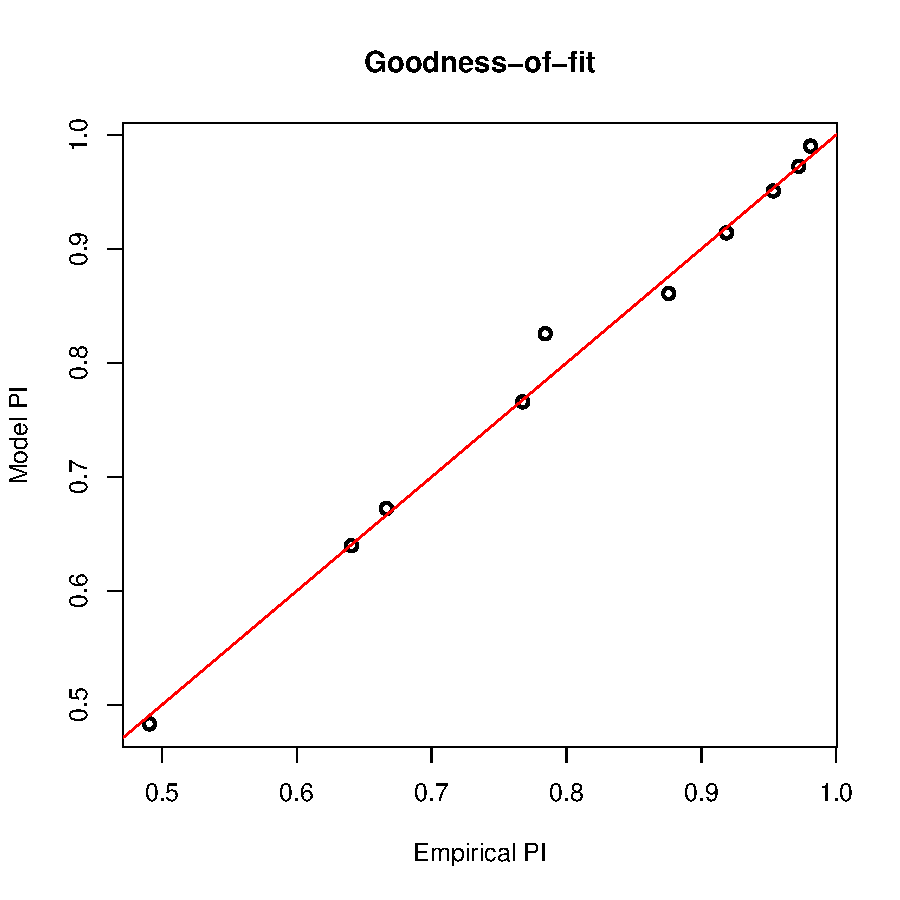
\includegraphics{pim-004}
\end{center}
The functions \texttt{coef()}, \texttt{vcov()} and \texttt{fitted.values()} provide the estimated coefficients, variance-covariance matrix of $\hat{\beta}$ and the fitted values respectively. 
\begin{Schunk}
\begin{Sinput}
> coef(pim.fit1)
\end{Sinput}
\begin{Soutput}
      Age_R-_L     Smoke_R-_L Age:Smoke_L-_R 
     0.6076003      5.3068852     -0.4553885 
\end{Soutput}
\begin{Sinput}
> vcov(pim.fit1)
\end{Sinput}
\begin{Soutput}
                    Age_R-_L   Smoke_R-_L Age:Smoke_L-_R
Age_R-_L        0.0009074760  0.009485251  -0.0009254122
Smoke_R-_L      0.0094852506  1.090409267  -0.0802054923
Age:Smoke_L-_R -0.0009254122 -0.080205492   0.0061690504
\end{Soutput}
\begin{Sinput}
> head(fitted.values(pim.fit1))
\end{Sinput}
\begin{Soutput}
            [,1]
26_222 0.5000000
26_23  0.6473932
222_23 0.6473932
26_59  0.6473932
222_59 0.6473932
23_59  0.5000000
\end{Soutput}
\end{Schunk}

We end this section with an illustration of the interpretation of the age effect. For 2 randomly selected children with the same smoking status and a year difference in age, the probability that the eldest has a higher FEV is estimated by $\text{expit}(0.61 - 0.46SMOKE)$. For non-smokers this probability is $0.65$, while for smokers this becomes $0.54$.

\section{Mental health study}

For the mental health study the following PIM was proposed
\begin{equation}\label{pim.mhs}
\text{logit}\left(\prob{MI \leqs MI'} \right) = \beta_1 (SES' - SES) + \beta_2 (LI' - LI). 
\end{equation}
\begin{Schunk}
\begin{Sinput}
> data("MHData")
> head(MHData)
\end{Sinput}
\begin{Soutput}
  mental ses life
1      1   1    1
2      1   1    9
3      1   1    4
4      1   1    3
5      1   0    2
6      1   1    0
\end{Soutput}
\end{Schunk}
Here \verb|mental| stands for the mental impairment ($MI$), \verb|ses| for the socioeconomic status ($SES$) and \verb|life| for the life index ($LI$). Similar as in the previous example we can specify a \texttt{lm()}-like formula. 
\begin{Schunk}
\begin{Sinput}
> pim.fit2a <- pim(mental ~ ses + life -1, data = MHData, link="logit", 
+ 								 poset=oldpimposet, estimator=estimator.nleqslv(ignore.error=TRUE), 
+ 								 keep.data=TRUE)
> summary(pim.fit2a)
\end{Sinput}
\begin{Soutput}
Call:
pim(frm = mental ~ ses + life - 1, data = MHData, link = "logit", 
    poset = oldpimposet, estimator = estimator.nleqslv(ignore.error = TRUE), 
    keep.data = TRUE)

           Estimate Std. Error Z value Pr(>|z|)   
ses_R-_L  -0.740163   0.343575 -2.1543 0.031217 * 
life_R-_L  0.201179   0.073371  2.7419 0.006108 **
---
Signif. codes:  0 '***' 0.001 '**' 0.01 '*' 0.05 '.' 0.1 ' ' 1 
\end{Soutput}
\end{Schunk}
The model is estimated by
\[
\text{logit}\left(\hatprob{MI \leqs MI'} \right) = -0.74 (SES' - SES) + 0.2 (LI' - LI). 
\]

Model (\ref{pim.mhs}) can be extended as follows
\begin{eqnarray*}
\text{logit}\left(\prob{MI \leqs MI'} \right) = \beta_1 (SES' - SES) + \beta_2 (LI' - LI) + \beta_3 SES + \beta_4 LI. 
\end{eqnarray*}
If we want to fit this model, we need to specify the \texttt{formula} statement explicitly because $Z$ is no longer of the form $Z = X' - X$. Some notation is needed to specify the predictors corresponding to the left response in $\prob{MI \leqs MI'}$, thus $(SES,LI)$ and the predictors corresponding to the right response, thus $(SES', LI')$. The altering functions can be used for this: \texttt{L()} for the predictors corresponding to the left response and \texttt{R()} for the predictors corresponding to the right response. Thus $(SES, LI)$ in R becomes \texttt{(L(ses), L(life)} and $(SES',LI')$ becomes \texttt{(R(ses), R(life)}. The \texttt{I()} statement is needed to specify specific functions. The function
\[
\beta_1 (SES' - SES) + \beta_2 (LI' - LI) + \beta_3 SES + \beta_4 LI,
\]
in R becomes
\begin{center}
\begin{verbatim}
 ~ ses + life + L(ses) + L(life) - 1
\end{verbatim}
\end{center}
\begin{Schunk}
\begin{Sinput}
> pim.fit2b <- pim(mental ~ ses + life + L(ses) + L(life) - 1, data = MHData, link="logit", 
+ 								 poset=oldpimposetbft, estimator=estimator.nleqslv(ignore.error=TRUE), 
+ 								 keep.data=TRUE)
> summary(pim.fit2b)
\end{Sinput}
\begin{Soutput}
Call:
pim(frm = mental ~ ses + life + L(ses) + L(life) - 1, data = MHData, 
    link = "logit", poset = oldpimposetbft, estimator = estimator.nleqslv(ignore.error = TRUE), 
    keep.data = TRUE)

           Estimate Std. Error Z value Pr(>|z|)   
ses_R-_L  -0.670723   0.382665 -1.7528 0.079642 . 
life_R-_L  0.205459   0.069989  2.9356 0.003329 **
ses_L     -0.034676   0.163157 -0.2125 0.831693   
life_L    -0.021601   0.039843 -0.5422 0.587711   
---
Signif. codes:  0 '***' 0.001 '**' 0.01 '*' 0.05 '.' 0.1 ' ' 1 
\end{Soutput}
\end{Schunk}
The estimated model is given by
\begin{eqnarray*}
\text{logit}\left(\hatprob{MI \leqs MI'} \right) = -0.67 (SES' - SES) + 0.21 (LI' - LI)  -0.03 SES  -0.02 LI. 
\end{eqnarray*}




\section{Food expenditure study}\label{S_fe}

Because of heteroscedasticity the following PIM is proposed to analyze the food expenditure data.
\[
\text{logit}\left( \prob{FE \leqs FE' } \right) = \beta \frac{HI' - HI}{\sqrt{HI' + HI}}.  
\]
\begin{Schunk}
\begin{Sinput}
> data("Engeldata")
\end{Sinput}
\end{Schunk}
Here \verb|income| denotes the household income ($HI$) while \verb|foodexp| denotes the food expenditure ($FE$). The covariate vector $Z$ is not of the form $Z = X' - X$, hence we need to specify the formula explicitly. 
\begin{Schunk}
\begin{Sinput}
> pim.fit3 <- pim(foodexp ~ I((R(income)-L(income))/sqrt(R(income)+L(income)))-1, 
+ 								data = Engeldata, link="logit", poset=oldpimposetbft, 
+ 								estimator=estimator.nleqslv(ignore.error=TRUE), 
+ 								keep.data=TRUE, 
+ 								extra.nicenames=data.frame(
+ 									org="I((R(income)-L(income))/sqrt(R(income)+L(income)))", 
+ 									nice="weightedincomediff", stringsAsFactors=FALSE))
> summary(pim.fit3)				
\end{Sinput}
\begin{Soutput}
Call:
pim(frm = foodexp ~ I((R(income) - L(income))/sqrt(R(income) + 
    L(income))) - 1, data = Engeldata, link = "logit", poset = oldpimposetbft, 
    estimator = estimator.nleqslv(ignore.error = TRUE), keep.data = TRUE, 
    extra.nicenames = data.frame(org = "I((R(income)-L(income))/sqrt(R(income)+L(income)))", 
        nice = "weightedincomediff", stringsAsFactors = FALSE))

                   Estimate Std. Error Z value  Pr(>|z|)    
weightedincomediff  0.38971    0.02436  15.998 < 2.2e-16 ***
---
Signif. codes:  0 '***' 0.001 '**' 0.01 '*' 0.05 '.' 0.1 ' ' 1 
\end{Soutput}
\end{Schunk}
The estimated model is given by 
\[
\text{logit}\left( \hatprob{FE \leqs FE' } \right) =  0.39 \frac{HI' - HI}{\sqrt{HI' + HI}}.  
\]



\section{Categorical predictors}\label{S_categorical}


In the presence of categorical predictors, a dummy coding is used together with the covariate vector $Z = X'_{dummy} - X_{dummy}$ , where $X_{dummy}$ denotes the dummy coding of the predictor $X$. This model is inspired by the relation between a linear models and a PIM. As an example consider a predictor $X$ with 3 levels $A$, $B$ and $C$ with dummy coding $X_{B} = 1$ if $X=B$ and $X_{B} = 0$ otherwise and $X_C = 1$ if $X = C$ and $X_C = 0$ otherwise. The linear model
\[
Y = \alpha_0 + \alpha_1 X_B + \alpha_2 X_C + \varepsilon,
\] 
with $\varepsilon \sim \text{N}(0,\sigma^2)$ embeds the PIM
\[
\prob{Y \leqs Y'| X, X'} = \Phi\left\{\beta_1 (X'_B - X_B) + \beta_2 (X'_C - X_C) \right\},
\]
where $\beta_i = \alpha_i/\sqrt{2 \sigma^2}$. Note that the PIM has only 2 parameters ($\beta_1$ and $\beta_2$) to model 3 probabilities $\prob{Y \leqs Y'| X = A, X' = B}$, $\prob{Y \leqs Y'| X = A, X' = C}$ and $\prob{Y \leqs Y'| X = B, X' = C}$. This is a consequence of the transitivity assumption which is implied by the linear model:
\begin{eqnarray*}
\prob{Y \leqs Y'| X = B, X' = C} &=& \Phi\left\{ \Phi^{-1} \left(\prob{Y \leqs Y'| X = A, X' = C} \right)  \right. \\
																 & & \left. 	- \Phi^{-1}\left(\prob{Y \leqs Y'| X = A, X' = B} \right) \right\}.
\end{eqnarray*}
In R this becomes
\begin{Schunk}
\begin{Sinput}
> n <- 100
> X <- factor(sample(LETTERS[1:3], n, replace = TRUE))
> Y <- model.matrix(~ X)%*%c(1,2,3) + rnorm(n)
> data.tmp <- data.frame(Y, X)
> pim.fit4 <- pim(Y ~ X-1, data = data.tmp, link = "probit", poset=oldpimposet, 
+ 								estimator=estimator.nleqslv(ignore.error=TRUE), keep.data=TRUE)
> summary(pim.fit4)
\end{Sinput}
\begin{Soutput}
Call:
pim(frm = Y ~ X - 1, data = data.tmp, link = "probit", poset = oldpimposet, 
    estimator = estimator.nleqslv(ignore.error = TRUE), keep.data = TRUE)

         Estimate Std. Error Z value  Pr(>|z|)    
X_R-_L_B  1.38692    0.20960   6.617 3.665e-11 ***
X_R-_L_C  2.05416    0.19683  10.436 < 2.2e-16 ***
---
Signif. codes:  0 '***' 0.001 '**' 0.01 '*' 0.05 '.' 0.1 ' ' 1 
\end{Soutput}
\end{Schunk}
The estimated model is given by
\[
\Phi^{-1}\left( \hatprob{Y \leqs Y'| X, X'} \right)= 1.39 (X'_B - X_B) + 2.05 (X'_C - X_C).
\]

Note that PIMs are semiparametric, thus the normality assumption is not required to obtain consistent and asymptotically normally distributed estimators. The linear model merely serves as a guide on how $Z$ can be constructed based on the predictors $X$ and $X'$.

\section{Conclusions and remarks}\label{S_conclusion}


The \texttt{pim}-package is illustrated on several examples and allows fitting a broad class of PIMs. PIMs which are embedded by a linear model as well as less restrictive PIMs are allowed. For categorical predictors however, only PIMs which are based on a linear model can be constructed.


Note that for a sample size of $n$ 	a total $n(n-1)/2$ pseudo-observations are created. Consequently for large sample sizes the function goes quite slow.  

In one of the next versions the above mentioned shortcomings will be tackled. All bugs/comments/suggestions are welcome at \href{mailto:JanR.DeNeve@Ugent.be}{JanR.DeNeve@Ugent.be}.


\bibliographystyle{plainnat}
\bibliography{jdeneve}

\end{document}
